\chapter{Создание электрической схемы} \label{chap:altium-SchDoc}

Так как схема большая, а места на листе мало, будем использовать иерархическую модель: схемы включения модулей изобразим на отдельных листах, а потом объединим их в общей схеме, используя элемент SheetSymbol.
\section{МШУ}

\begin{figure}[H]
	\centering
	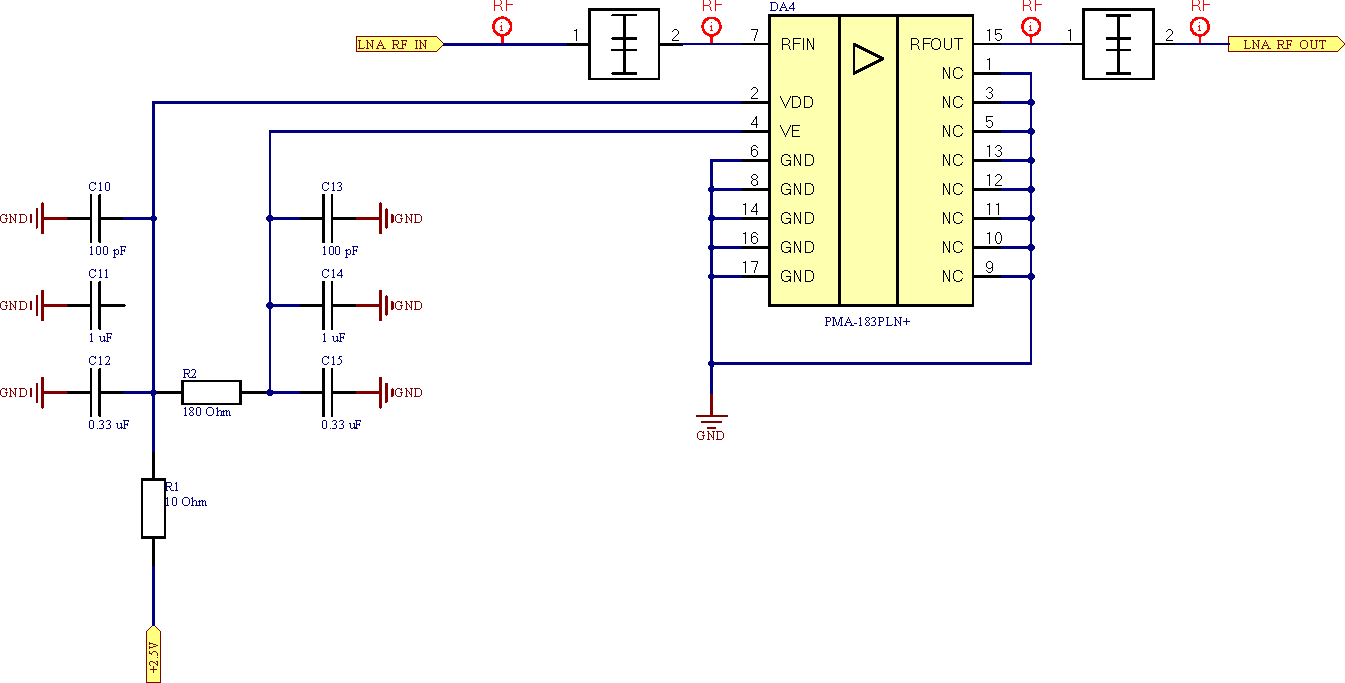
\includegraphics[width=0.95\textwidth]{LNA_SchDoc.pdf}
	\caption{Схема включения МШУ}%
	\label{fig:LNA-SchDoc}
\end{figure}

\section{Детектор мощности}

\begin{figure}[H]
	\centering
	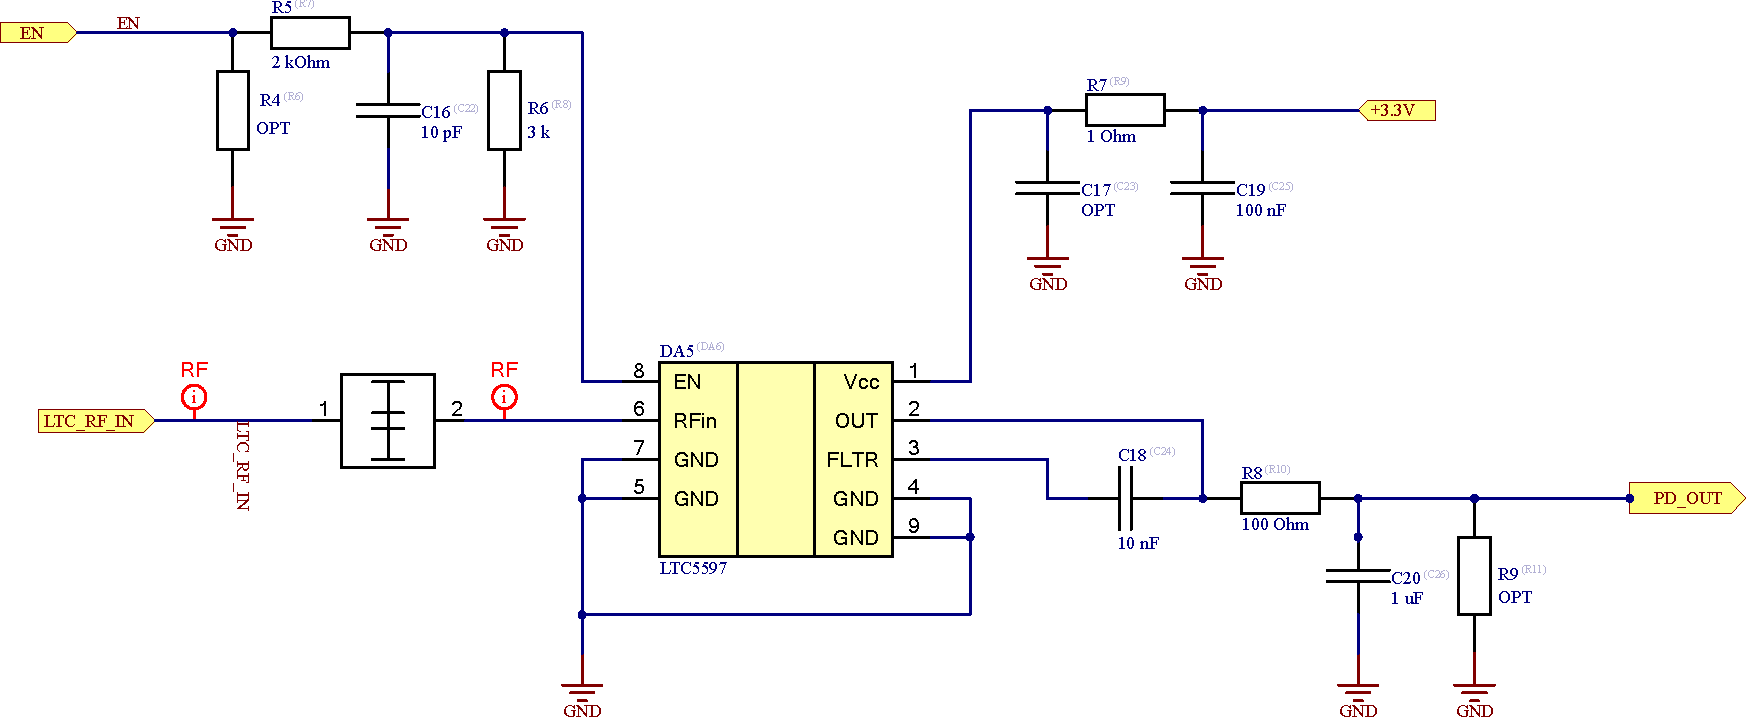
\includegraphics[width=0.95\textwidth]{PD_SchDoc.pdf}
	\caption{Схема включения детектора мощности}%
	\label{fig:PD-SchDoc}
\end{figure}

Также на данной схеме обозначены входы АЦП микроконтроллера.

\section{Микроконтроллер}

\begin{figure}[H]
	\centering
	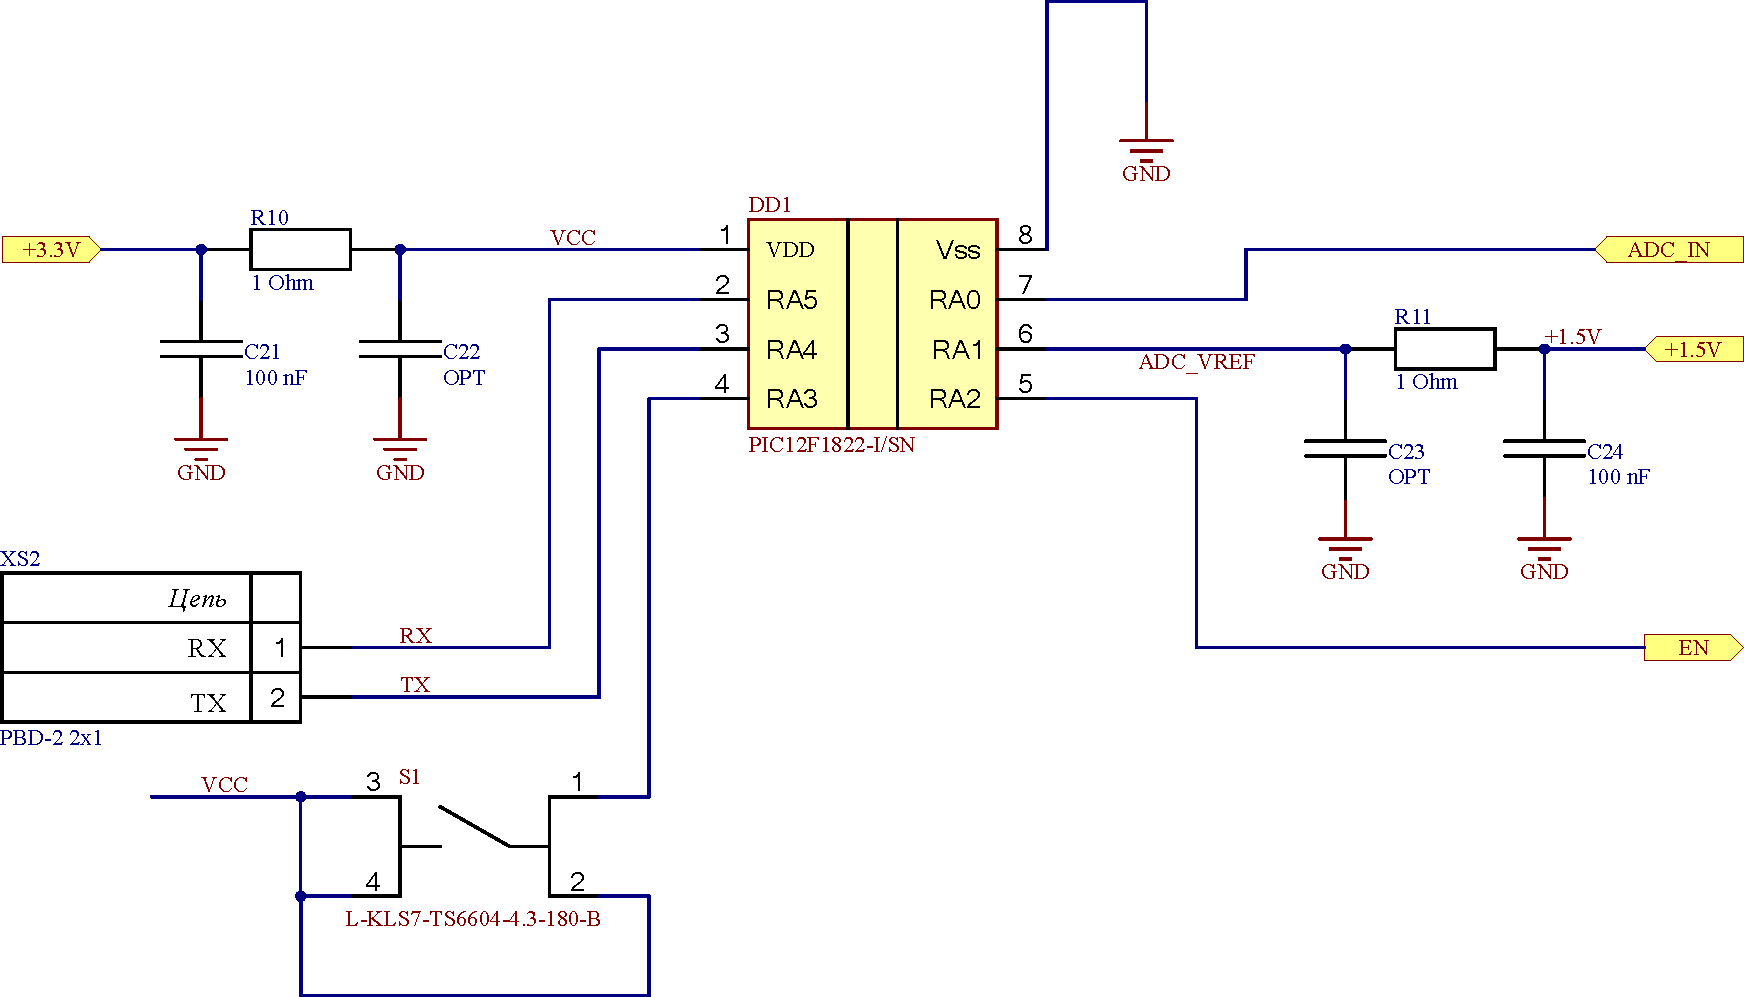
\includegraphics[width=0.95\textwidth]{MC_SchDoc.pdf}
	\caption{Схема включения микроконтроллера}%
	\label{fig:MC-SchDoc}
\end{figure}

\section{Питание}

\begin{figure}[H]
	\centering
	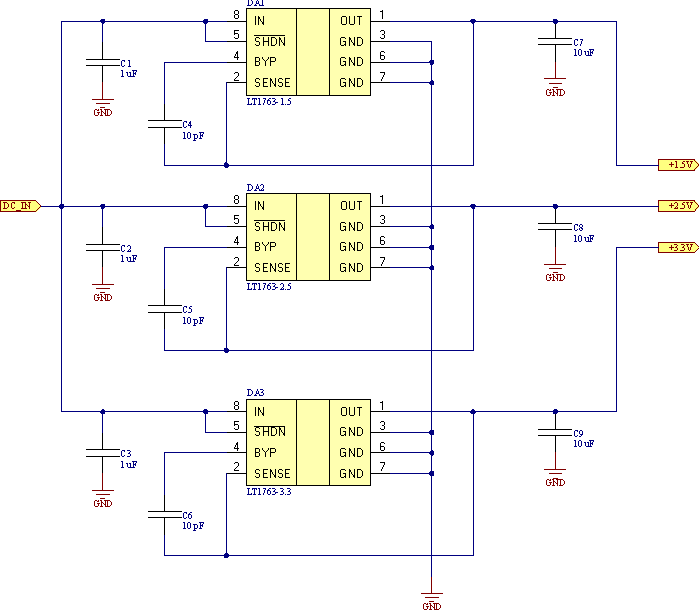
\includegraphics[width=0.95\textwidth]{PM_SchDoc.pdf}
	\caption{Схема включения преобразователей напряжения}%
	\label{fig:PM-SchDoc}
\end{figure}

\section{Общий вид}

\begin{figure}[H]
	\centering
	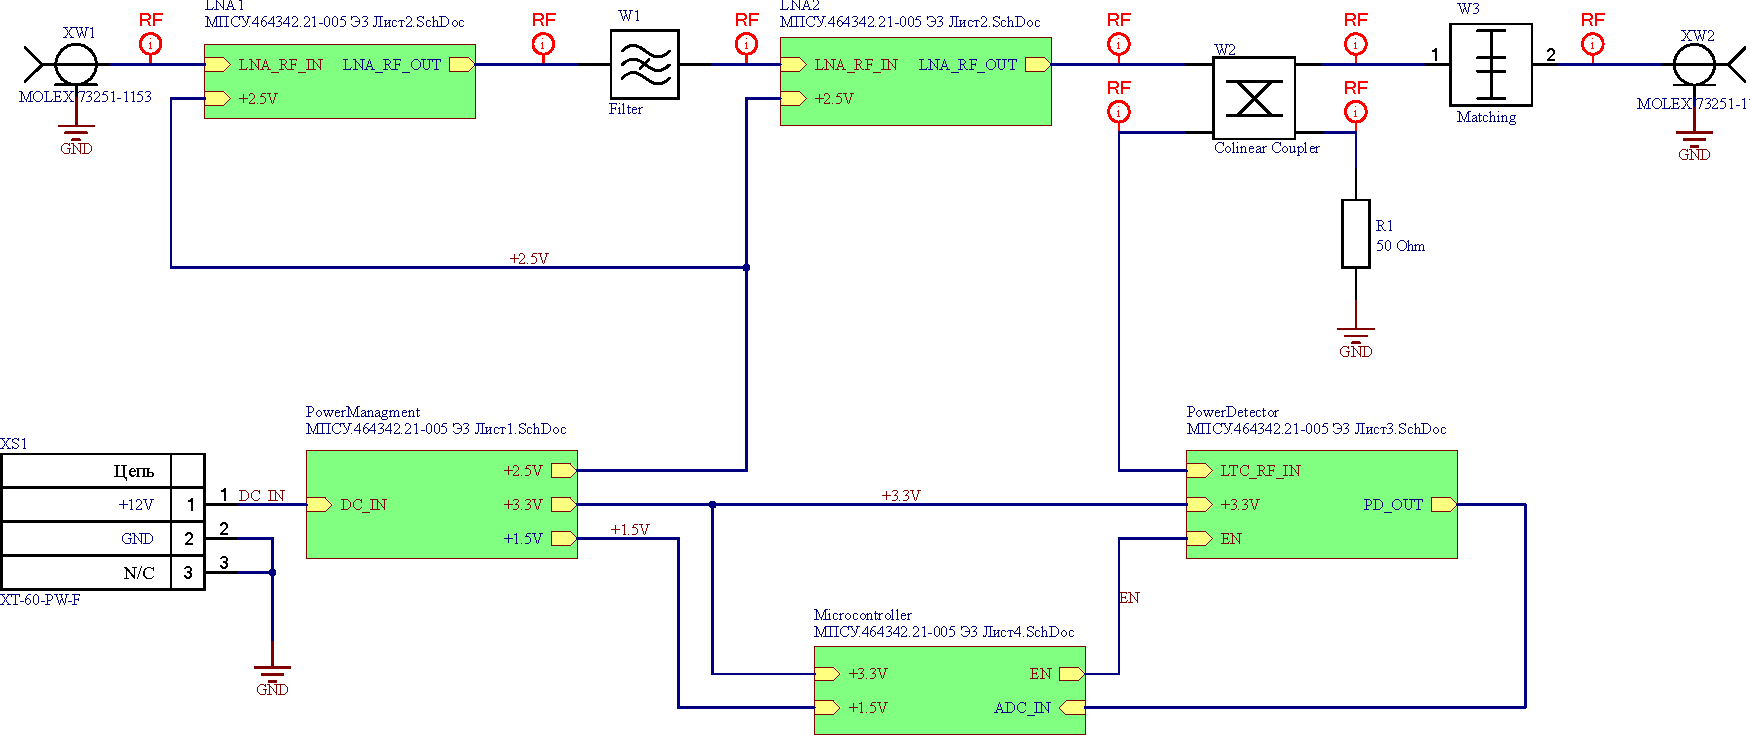
\includegraphics[width=0.95\textwidth]{Main_SchDoc.pdf}
	\caption{Главная схема}%
	\label{fig:Main_SchDoc}
\end{figure}

Дополнительно зададим классы для ВЧ линий и элементов. (потому что со схематика это проше сделать.)